\documentclass[12pt, fullpage,letterpaper]{article}

\usepackage[margin=1in]{geometry}
\usepackage{url}
\usepackage{amsmath}
\usepackage{amssymb}
\usepackage{xspace}
\usepackage{graphicx}
\usepackage{bm}

%table position
\usepackage{float}
%multi columns
\usepackage[english]{babel}
\usepackage{multicol}
%caption without figure number
\usepackage{caption}
%drawing trees
\usepackage{tikz}
\usetikzlibrary{calc, shapes, backgrounds}
%merge cells
\usepackage{booktabs}
\usepackage{multirow}

\newcommand{\semester}{Spring 2018}
\newcommand{\assignmentId}{1}

\newcommand{\bx}{{\bf x}}
\newcommand{\bw}{{\bf w}}

\title{CS 5350/6350: Machine Learining \semester}
\author{Homework \assignmentId\ Solutions\\\\Yulong Liang (u1143816)}

\begin{document}
\maketitle

\section{Hypothesis Space}

\begin{enumerate}
\item~[30 points] Conjunctions:

\begin{enumerate}
\item \textbf{Answer:}
\begin{multicols}{3}
$\Phi$ (Always False)\\
$x_1$\\
$\neg x_1$\\
$x_2$\\
$\neg x_2$\\
$x_3$\\
$\neg x_3$\\
$x_4$\\
$\neg x_4$\\
$x_1 \wedge x_2$\\
$\neg x_1 \wedge x_2$\\
$x_1 \wedge \neg x_2$\\
$\neg x_1 \wedge \neg x_2$\\
$x_1 \wedge x_3$\\
$\neg x_1 \wedge x_3$\\
$x_1 \wedge \neg x_3$\\
$\neg x_1 \wedge \neg x_3$\\
$x_1 \wedge x_4$\\
$\neg x_1 \wedge x_4$\\
$x_1 \wedge \neg x_4$\\
$\neg x_1 \wedge \neg x_4$\\
$x_2 \wedge x_3$\\
$\neg x_2 \wedge x_3$\\
$x_2 \wedge \neg x_3$\\
$\neg x_2 \wedge \neg x_3$\\
$x_2 \wedge x_4$\\
$\neg x_2 \wedge x_4$\\
$x_2 \wedge \neg x_4$\\
$\neg x_2 \wedge \neg x_4$\\
$x_3 \wedge x_4$\\
$\neg x_3 \wedge x_4$\\
$x_3 \wedge \neg x_4$\\
$\neg x_3 \wedge \neg x_4$\\
$x_1 \wedge x_2 \wedge x_3$\\
$\neg x_1 \wedge x_2 \wedge x_3$\\
$x_1 \wedge \neg x_2 \wedge x_3$\\
$x_1 \wedge x_2 \wedge \neg x_3$\\
$\neg x_1 \wedge \neg x_2 \wedge x_3$\\
$x_1 \wedge \neg x_2 \wedge \neg x_3$\\
$\neg x_1 \wedge x_2 \wedge \neg x_3$\\
$\neg x_1 \wedge \neg x_2 \wedge \neg x_3$\\
$x_1 \wedge x_2 \wedge x_4$\\
$\neg x_1 \wedge x_2 \wedge x_4$\\
$x_1 \wedge \neg x_2 \wedge x_4$\\
$x_1 \wedge x_2 \wedge \neg x_4$\\
$\neg x_1 \wedge \neg x_2 \wedge x_4$\\
$x_1 \wedge \neg x_2 \wedge \neg x_4$\\
$\neg x_1 \wedge x_2 \wedge \neg x_4$\\
$\neg x_1 \wedge \neg x_2 \wedge \neg x_4$\\
$x_1 \wedge x_3 \wedge x_4$\\
$\neg x_1 \wedge x_3 \wedge x_4$\\
$x_1 \wedge \neg x_3 \wedge x_4$\\
$x_1 \wedge x_3 \wedge \neg x_4$\\
$\neg x_1 \wedge \neg x_3 \wedge x_4$\\
$x_1 \wedge \neg x_3 \wedge \neg x_4$\\
$\neg x_1 \wedge x_3 \wedge \neg x_4$\\
$\neg x_1 \wedge \neg x_3 \wedge \neg x_4$\\
$x_2 \wedge x_3 \wedge x_4$\\
$\neg x_2 \wedge x_3 \wedge x_4$\\
$x_2 \wedge \neg x_3 \wedge x_4$\\
$x_2 \wedge x_3 \wedge \neg x_4$\\
$\neg x_2 \wedge \neg x_3 \wedge x_4$\\
$x_2 \wedge \neg x_3 \wedge \neg x_4$\\
$\neg x_2 \wedge x_3 \wedge \neg x_4$\\
$\neg x_2 \wedge \neg x_3 \wedge \neg x_4$\\
$x_1 \wedge x_2 \wedge x_3 \wedge x_4$\\
$\neg x_1 \wedge x_2 \wedge x_3 \wedge x_4$\\
$x_1 \wedge \neg x_2 \wedge x_3 \wedge x_4$\\
$x_1 \wedge x_2 \wedge \neg x_3 \wedge x_4$\\
$x_1 \wedge x_2 \wedge x_3 \wedge \neg x_4$\\
$\neg x_1 \wedge \neg x_2 \wedge x_3 \wedge x_4$\\
$\neg x_1 \wedge x_2 \wedge \neg x_3 \wedge x_4$\\
$\neg x_1 \wedge x_2 \wedge x_3 \wedge \neg x_4$\\
$x_1 \wedge \neg x_2 \wedge \neg x_3 \wedge x_4$\\
$x_1 \wedge \neg x_2 \wedge x_3 \wedge \neg x_4$\\
$x_1 \wedge x_2 \wedge \neg x_3 \wedge \neg x_4$\\
$\neg x_1 \wedge \neg x_2 \wedge \neg x_3 \wedge x_4$\\
$\neg x_1 \wedge \neg x_2 \wedge x_3 \wedge \neg x_4$\\
$x_1 \wedge \neg x_2 \wedge \neg x_3 \wedge \neg x_4$\\
$\neg x_1 \wedge \neg x_2 \wedge \neg x_3 \wedge \neg x_4$\\
\end{multicols}
\item \textbf{Answer:}\\
$\neg x_2 \wedge x_4$
\item \textbf{Answer:}\\
$3^n$(each variable can be positive, negative or nothing)
\item \textbf{Answer:}\\
$2^{2^n}=4^n$
\end{enumerate}

\item~ [30 points] m-of-n rules:
\begin{enumerate}
\item \textbf{Answer:}
\begin{multicols}{2}
Always false\\
at least 1 of $\{x_1\}$ are 1\\
at least 1 of $\{x_2\}$ are 1\\
at least 1 of $\{x_3\}$ are 1\\
at least 1 of $\{x_4\}$ are 1\\
at least 1 of $\{x_1, x_2\}$ are 1\\
at least 2 of $\{x_1, x_2\}$ are 1\\
at least 1 of $\{x_1, x_3\}$ are 1\\
at least 2 of $\{x_1, x_3\}$ are 1\\
at least 1 of $\{x_1, x_4\}$ are 1\\
at least 2 of $\{x_1, x_4\}$ are 1\\
at least 1 of $\{x_2, x_3\}$ are 1\\
at least 2 of $\{x_2, x_3\}$ are 1\\
at least 1 of $\{x_2, x_4\}$ are 1\\
at least 2 of $\{x_2, x_4\}$ are 1\\
at least 1 of $\{x_3, x_4\}$ are 1\\
at least 2 of $\{x_3, x_4\}$ are 1\\
at least 1 of $\{x_1, x_2, x_3\}$ are 1\\
at least 2 of $\{x_1, x_2, x_3\}$ are 1\\
at least 3 of $\{x_1, x_2, x_3\}$ are 1\\
at least 1 of $\{x_1, x_2, x_4\}$ are 1\\
at least 2 of $\{x_1, x_2, x_4\}$ are 1\\
at least 3 of $\{x_1, x_2, x_4\}$ are 1\\
at least 1 of $\{x_1, x_3, x_4\}$ are 1\\
at least 2 of $\{x_1, x_3, x_4\}$ are 1\\
at least 3 of $\{x_1, x_3, x_4\}$ are 1\\
at least 1 of $\{x_2, x_3, x_4\}$ are 1\\
at least 2 of $\{x_2, x_3, x_4\}$ are 1\\
at least 3 of $\{x_2, x_3, x_4\}$ are 1\\
at least 1 of $\{x_1, x_2, x_3, x_4\}$ are 1\\
at least 2 of $\{x_1, x_2, x_3, x_4\}$ are 1\\
at least 3 of $\{x_1, x_2, x_3, x_4\}$ are 1\\
at least 4 of $\{x_1, x_2, x_3, x_4\}$ are 1\\
Always True
\end{multicols}
\item \textbf{Answer:}\\
at least 2 of $\{x_1, x_3, x_4\}$ are 1
\item \textbf{Answer:}\\
$\sum_{i=0}^n i{n \choose i}=n\cdot2^{n-1}$
\item \textbf{Answer:}\\
No, it's not. The m-of-n rule has a smaller hypothesis space than conjunctions.
\end{enumerate}
\end{enumerate}

\section{Decision Tree}
\begin{enumerate}
\item~[20 points]
\begin{enumerate}
\item \textbf{Answer:}
\begin{itemize}
\item \textbf{Step 1}\\
Current Entropy,
$$H=-(\frac{2}{7}\log_2\frac{2}{7}+\frac{5}{7}\log_2\frac{5}{7})=0.8631$$
Expected Entropy,
\begin{align*}
H_{x_1}&=\frac{5}{7} \cdot [-(\frac{1}{5}\log_2\frac{1}{5}+\frac{4}{5}\log_2\frac{4}{5})] + \frac{2}{7} \cdot [-(\frac{1}{2}\log_2\frac{1}{2}+\frac{1}{2}\log_2\frac{1}{2})]\\
&=0.8014\\
H_{x_2}&=\frac{3}{7} \cdot [-(\frac{1}{3}\log_2\frac{1}{3}+\frac{2}{3}\log_2\frac{2}{3})] + \frac{4}{7} \cdot [-(1\log_21)]\\
&=0.3936\\
H_{x_3}&=\frac{4}{7} \cdot [-(\frac{1}{4}\log_2\frac{1}{4}+\frac{3}{4}\log_2\frac{3}{4})] + \frac{3}{7} \cdot [-(\frac{1}{3}\log_2\frac{1}{3}+\frac{2}{3}\log_2\frac{2}{3})]\\
&=0.8571\\
H_{x_4}&=\frac{4}{7} \cdot [-(1\log_21)] + \frac{3}{7} \cdot [-(\frac{2}{3}\log_2\frac{2}{3}+\frac{1}{3}\log_2\frac{1}{3})]\\
&=0.3936
\end{align*}
Expected Information Gain,
$$Gain_{x_1}=H-H_{x_1}=0.8631-0.8014=0.0617$$
$$Gain_{x_2}=H-H_{x_2}=0.8631-0.3936=0.4695$$
$$Gain_{x_3}=H-H_{x_3}=0.8631-0.8571=0.0060$$
$$Gain_{x_4}=H-H_{x_4}=0.8631-0.3936=0.4695$$
Thus, we split attribute $x_2$.
\item \textbf{Step 2}\\
For $x_2=0$, the data subset is as follows,
\begin{table}[H]
\centering
\begin{tabular}{ccc|c}
$x_1$&$x_3$&$x_4$&$y$\\
\hline \hline
0&1&0&0\\
0&1&1&1\\
1&0&1&1\\
\end{tabular}
\end{table}
Current Entropy,
$$H=-(\frac{1}{3}\log_2\frac{1}{3}+\frac{2}{3}\log_2\frac{2}{3})=0.9183$$
Expected Entropy,
\begin{align*}
H_{x_1}&=\frac{2}{3} \cdot [-(\frac{1}{2}\log_2\frac{1}{2}+\frac{1}{2}\log_2\frac{1}{2})] + \frac{1}{3} \cdot [-(1\log_21)]\\
&=0.6667\\
H_{x_3}&=\frac{1}{3} \cdot [-(1\log_21)] + \frac{2}{3} \cdot [-(\frac{1}{2}\log_2\frac{1}{2}+\frac{1}{2}\log_2\frac{1}{2})]\\
&=0.6667\\
H_{x_4}&=2\cdot(-1\log_21)\\
&=0
\end{align*}
Expected Information Gain,
$$Gain_{x_1}=H-H_{x_1}=0.9183-0.6667=0.2516$$
$$Gain_{x_3}=H-H_{x_3}=0.9183-0.6667=0.2516$$
$$Gain_{x_4}=H-H_{x_4}=0.9183-0=0.9183$$
Thus, we split attribute $x_4$.\\
For $x_2=1$, the data subset is as follows,
\begin{table}[H]
\centering
\begin{tabular}{ccc|c}
$x_1$&$x_3$&$x_4$&$y$\\
\hline \hline
0&0&0&0\\
0&1&0&0\\
1&0&0&0\\
0&0&1&0\\
\end{tabular}
\end{table}
Thus, the data is pure. We can create a leaf node and assign 0 as the label.
\item \textbf{Step 3}
For $x_2=0$ and $x_4=0$, the data subset is as follows,
\begin{table}[H]
\centering
\begin{tabular}{cc|c}
$x_1$&$x_3$&$y$\\
\hline \hline
0&1&0\\
\end{tabular}
\end{table}
Thus, the data is pure. We can create a leaf node and assign 0 as the label.\\
For $x_2=0$ and $x_4=1$, the data subset is as follows,
\begin{table}[H]
\centering
\begin{tabular}{cc|c}
$x_1$&$x_3$&$y$\\
\hline \hline
0&1&1\\
1&0&1\\
\end{tabular}
\end{table}
Thus, the data is pure. We can create a leaf node and assign 1 as the label.\\\\
Since all the branches reach the leaf node, the tree is constructed successfully,
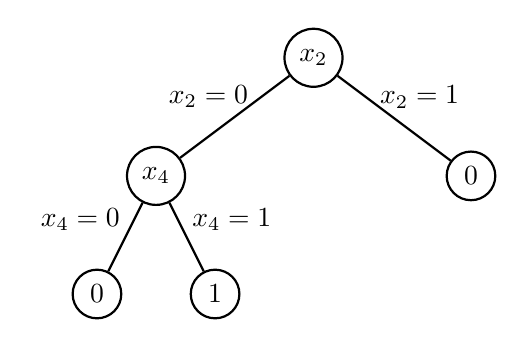
\begin{tikzpicture}
  [
    scale = 1, transform shape, thick,
    every node/.style = {draw, circle},
    grow = down,  % alignment of characters
    level 1/.style = {sibling distance=4cm},
    level 2/.style = {sibling distance=1.5cm}, 
    level distance = 1.5cm
  ]
  \node (Start) {$x_2$} 
   child { node (A) {$x_4$}
     child { node (B) {0}}
     child { node (C) {1}}
   }
   child { node (D) {0}
   };
  \begin{scope}[nodes = {draw = none}]
    \path (Start) -- (A) node [near start, left]  {$x_2=0$};
    \path (Start) -- (D) node [near start, right] {$x_2=1$};
    \path (A) -- (B) node [near start, left]  {$x_4=0$};
    \path (A) -- (C) node [near start, right] {$x_4=1$};
  \end{scope}
\end{tikzpicture}
\end{itemize}
\item \textbf{Answer:}
\begin{table}[H]
\centering
\begin{tabular}{cccc|c}
$x_1$&$x_2$&$x_3$&$x_4$&$y$\\
\hline \hline
0&0&0&0&0\\
0&0&0&1&1\\
0&0&1&0&0\\
0&0&1&1&1\\
0&1&0&0&0\\
0&1&0&1&0\\
0&1&1&0&0\\
0&1&1&1&0\\
1&0&0&0&0\\
1&0&0&1&1\\
1&0&1&0&0\\
1&0&1&1&1\\
1&1&0&0&0\\
1&1&0&1&0\\
1&1&1&0&0\\
1&1&1&1&0\\
\end{tabular}
\end{table}
\item \textbf{Answer:}\\
Because \texttt{ID3 Algorithm} is a greedy heuristic algorithm. It will not try to explore the entire hypothesis space and find the optimal result. Each step of the iteration will guarantee to find the purest way to split the data for that particular step. The overall solution may not be the best, but will be a pretty good one.
\end{enumerate}
\item~[20 points]
\begin{enumerate}
\item \textbf{Answer:}
\begin{itemize}
\item \textbf{Step 1}\\
Current Entropy,
$$H=-(\frac{2}{12}\log_2\frac{2}{12}+\frac{7}{12}\log_2\frac{7}{12}+\frac{3}{12}\log_2\frac{3}{12})=1.3844$$
Expected Entropy,
\begin{align*}
H_{shape}=&\frac{6}{12} \cdot [-(\frac{2}{6}\log_2\frac{2}{6}+\frac{2}{6}\log_2\frac{2}{6}+\frac{2}{6}\log_2\frac{2}{6})]+\frac{2}{12} \cdot [-(1\log_21)]+\\
&\frac{4}{12} \cdot [-(\frac{3}{4}\log_2\frac{3}{4}+\frac{1}{4}\log_2\frac{1}{4})]\\
=&1.0635\\
H_{color}=&\frac{3}{12} \cdot [-(1\log_21)]+\frac{4}{12} \cdot [-(\frac{2}{4}\log_2\frac{2}{4}+\frac{2}{4}\log_2\frac{2}{4})]+\\
&\frac{5}{12} \cdot [-(\frac{2}{5}\log_2\frac{2}{5}+\frac{2}{5}\log_2\frac{2}{5}+\frac{1}{5}\log_2\frac{1}{5})]\\
=&0.9675
\end{align*}
Expected Information Gain,
$$Gain_{shape}=H-H_{shape}=1.3844-1.0635=0.3209$$
$$Gain_{color}=H-H_{color}=1.3844-0.9675=0.4169$$
Thus, we split attribute \textbf{color}.
\item \textbf{Step 2}\\
For color=red, the data is pure. We can assign the label as B.\\
For color=green, the data is not pure. We continue split with the remaining attribute \textbf{shape}.\\
For color=blue, the data is not pure. We continue split with the remaining attribute \textbf{shape}.
\item \textbf{Step 3}\\
For color=green and shape=circle, all the data are labeled as A. Thus we can create a leaf node with label A.\\
For color=green and shape=square, all the data are labeled as B. Thus we can create a leaf node with label B.\\
For color=green and shape=triangle, there are no data. Thus we create a leaf node and assign the most common label in color=green. For this particular case, label A and label B are equally frequent. Thus we can assign the either of them. I will assign label B.\\
For color=blue and shape=circle, all the data are labeled as C. Thus we can create a leaf node with label C.\\
For color=blue and shape=square, all the data are labeled as A. Thus we can create a leaf node with label A.\\
For color=blue and shape=triangle, all the data are labeled as B. Thus we can create a leaf node with label B.\\\\
Since all the branches reach the leaf node, the tree is constructed successfully,
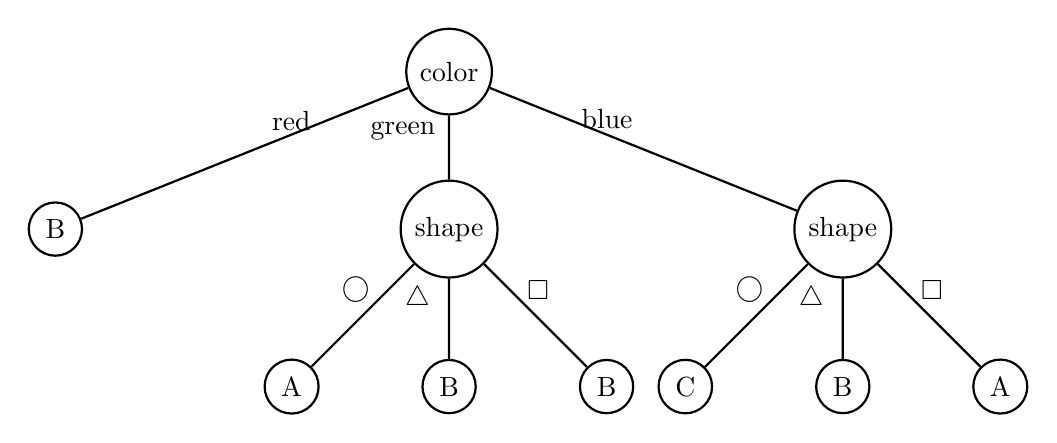
\begin{tikzpicture}
  [
    scale = 1, transform shape, thick,
    every node/.style = {draw, circle},
    grow = down,  % alignment of characters
    level 1/.style = {sibling distance=5cm},
    level 2/.style = {sibling distance=2cm}, 
    level distance = 2cm
  ]
  \node (Start) {color} 
   child { node (A) {B}}
   child { node (B) {shape}
     child { node (BA) {A}}
     child { node (BB) {B}}
     child { node (BC) {B}}
   }
   child { node (C) {shape}
     child { node (CA) {C}}
     child { node (CB) {B}}
     child { node (CC) {A}}};
  \begin{scope}[nodes = {draw = none}]
    \path (Start) -- (A) node [near start, left]  {red};
    \path (Start) -- (B) node [near start, left] {green};
    \path (Start) -- (C) node [near start, right] {blue};
    \path (B) -- (BA) node [near start, left]  {$\bigcirc$};
    \path (B) -- (BB) node [near start, left]  {$\triangle$};
    \path (B) -- (BC) node [near start, right]  {$\square$};
    \path (C) -- (CA) node [near start, left]  {$\bigcirc$};
    \path (C) -- (CB) node [near start, left]  {$\triangle$};
    \path (C) -- (CC) node [near start, right]  {$\square$};
  \end{scope}
\end{tikzpicture}
\end{itemize}
\item \textbf{Answer:}\\
Label B. (Label A is also reasonable because they are equally common.)
\item \textbf{Answer:}\\
My tree take the corner case where the example set is empty into consideration. Namely, create a leaf node with the most common label in the upper level example set. However, the example tree does nothing when it encounter an empty example set.
\end{enumerate}
\item~[20 points]
\begin{enumerate}
\item \textbf{Answer:}\\
The most common value for O(utlook) is S(unny) or R(ainy), both of which have 5 examples. I will pick S(unny) as the missing value.\\
Current Entropy,
$$H=-(\frac{5}{15}\log_2\frac{5}{15}+\frac{10}{15}\log_2\frac{10}{15})=0.9183$$
Expected Entropy,
\begin{align*}
H_{Outlook}=&\frac{6}{15} \cdot [-(\frac{3}{6}\log_2\frac{3}{6}+\frac{3}{6}\log_2\frac{3}{6})]+\frac{4}{15} \cdot [-1\log_21]+\\
&\frac{5}{15} \cdot [-(\frac{3}{5}\log_2\frac{3}{5}+\frac{2}{5}\log_2\frac{2}{5})]\\
=&0.7237\\
H_{Temperature}=&\frac{4}{15} \cdot [-(\frac{2}{4}\log_2\frac{2}{4}+\frac{2}{4}\log_2\frac{2}{4})]+\frac{7}{15} \cdot [-(\frac{2}{7}\log_2\frac{2}{7}+\frac{5}{7}\log_2\frac{5}{7})]+\\
&\frac{4}{15} \cdot [-(\frac{3}{4}\log_2\frac{3}{4}+\frac{1}{4}\log_2\frac{1}{4})]\\
=&0.8858\\
H_{Humidity}=&\frac{7}{15} \cdot [-(\frac{3}{7}\log_2\frac{3}{7}+\frac{4}{7}\log_2\frac{4}{7})]+\frac{8}{15} \cdot [-(\frac{1}{8}\log_2\frac{1}{8}+\frac{7}{8}\log_2\frac{7}{8})]\\
=&0.7497\\
H_{Wind}=&\frac{9}{15} \cdot [-(\frac{7}{9}\log_2\frac{7}{9}+\frac{2}{9}\log_2\frac{2}{9})]+\frac{6}{15} \cdot [-(\frac{3}{6}\log_2\frac{3}{6}+\frac{3}{6}\log_2\frac{3}{6})]\\
=&0.8585\\
\end{align*}
Expected Information Gain,
$$Gain_{Outlook}=H-H_{Outlook}=0.9183-0.7237=0.1946$$
$$Gain_{Temperature}=H-H_{Temperature}=0.9183-0.8858=0.0325$$
$$Gain_{Humidity}=H-H_{Humidity}=0.9183-0.7497=0.1686$$
$$Gain_{Wind}=H-H_{Wind}=0.9183-0.8585=0.0598$$
\item \textbf{Answer:}\\
The most common value with the same label for O(utlook) is O(vercast), which has 4 examples.\\
Current Entropy $H=0.9183$ and entropies $H_{Temperature}=0.8858$, $H_{Humidity}=0.7497$, $H_{Wind}=0.7497$ remain the same as \texttt{answer(a)}.\\
Expected Entropy for Outlook,
\begin{align*}
H_{Outlook}=&\frac{5}{15} \cdot [-(\frac{3}{5}\log_2\frac{3}{5}+\frac{2}{5}\log_2\frac{2}{5})]+\frac{5}{15} \cdot [-1\log_21]+\\
&\frac{5}{15} \cdot [-(\frac{3}{5}\log_2\frac{3}{5}+\frac{2}{5}\log_2\frac{2}{5})]\\
=0.6473&
\end{align*}
Expected Information Gain,
$$Gain_{Outlook}=H-H_{Outlook}=0.9183-0.6473=0.2710$$
$$Gain_{Temperature}=H-H_{Temperature}=0.9183-0.8858=0.0325$$
$$Gain_{Humidity}=H-H_{Humidity}=0.9183-0.7497=0.1686$$
$$Gain_{Wind}=H-H_{Wind}=0.9183-0.8585=0.0598$$
\item \textbf{Answer:}\\
For all the examples, there are $\frac{5}{14}$ S(unny), $\frac{4}{14}$ O(vercast), and $\frac{5}{14}$ R(ainy). We split the missing data and add fractional counts to the each possible value, namely $\frac{5}{14}$ S(unny) +, $\frac{4}{14}$ O(vercast) +, and $\frac{5}{14}$ R(ainy) +.\\
Current Entropy $H=0.9183$ and entropies $H_{Temperature}=0.8858$, $H_{Humidity}=0.7497$, $H_{Wind}=0.7497$ remain the same as \texttt{answer(a)}.\\
Expected Entropy for Outlook,
\begin{align*}
H_{Outlook}=&\frac{5+\frac{5}{14}}{15} \cdot [-(\frac{2+\frac{5}{14}}{5+\frac{5}{14}}\log_2\frac{2+\frac{5}{14}}{5+\frac{5}{14}}+\frac{3}{5+\frac{5}{14}}\log_2\frac{3}{5+\frac{5}{14}})]+\\
&\frac{4+\frac{4}{14}}{15} \cdot [-1\log_21]+\\
&\frac{5+\frac{5}{14}}{15} \cdot [-(\frac{3+\frac{5}{14}}{5+\frac{5}{14}}\log_2\frac{3+\frac{5}{14}}{5+\frac{5}{14}}+\frac{2}{5+\frac{5}{14}}\log_2\frac{2}{5+\frac{5}{14}})]+\\
=&0.6939
\end{align*}
Expected Information Gain,
$$Gain_{Outlook}=H-H_{Outlook}=0.9183-0.6939=0.2244$$
$$Gain_{Temperature}=H-H_{Temperature}=0.9183-0.8858=0.0325$$
$$Gain_{Humidity}=H-H_{Humidity}=0.9183-0.7497=0.1686$$
$$Gain_{Wind}=H-H_{Wind}=0.9183-0.8585=0.0598$$
\end{enumerate}
\item \textbf{Answer:}
\begin{align}
Gain(S,A)=&H(S)-H(S|A)\\
=&\sum_{s\in S}-p(s)\log_2p(s)-\sum_{a\in A}p(a)\sum_{s\in S}-p(s|a)\log_2p(s|a)\\
=&\sum_{a\in A}p(a)\sum_{s\in S}p(s|a)\log_2p(s|a)-\sum_{s\in S}p(s)\log_2p(s)\\
=&\sum_{a\in A}\sum_{s\in S}p(a)p(s|a)\log_2p(s|a)-\sum_{s\in S}\sum_{a\in A}p(s,a)\log_2p(s)\\
=&\sum_{a\in A}\sum_{s\in S}p(s,a)\log_2p(s|a)-\sum_{s\in S}\sum_{a\in A}p(s,a)\log_2p(s)\\
=&\sum_{a\in A}\sum_{s\in S}p(s,a)\big[\log_2p(s|a)-\log_2p(s)\big]\\
=&-\sum_{a\in A}\sum_{s\in S}p(s,a)\big[\log_2\frac{p(s)}{p(s|a)}\big]\\
=&-\sum_{a\in A}p(a)\sum_{s\in S}p(s|a)\big[\log_2\frac{p(s)}{p(s|a)}\big]
\end{align}
Let $f(x)=\log_2x$, then $f'(x)=\cfrac{1}{x\ln2}>0.\quad\therefore f(x)=\log2_x$ is convex.\\
According to Jensen’s inequality, 
\begin{align}
\sum_xp(x)&f(x) \leq f(\sum_xp(x)x)\\
Gain(S,A)=&-\sum_{a\in A}p(a)\sum_{s\in S}p(s|a)\big[\log_2\frac{p(s)}{p(s|a)}\big]\\
\geq&-\sum_{a\in A}p(a)\big[\log_2\sum_{s\in S}\frac{p(s|a)p(s)}{p(s|a)}\big]\\
\geq&-\log_2\big[\sum_{a\in A}\sum_{s\in S}\frac{p(s|a)p(s)p(a)}{p(s|a)}\big]\\
=&-\log_2\big[\sum_{a\in A}p(a)\sum_{s\in S}p(s)\big]\\
=&-\log_21\\
=&0
\end{align}
\end{enumerate}

\section{Programming Assignments}

\begin{enumerate}
\setcounter{enumi}{1}
\item \textbf{Answer:}\\
\begin{table}[H]
\centering
\begin{tabular}{c|cccc}
\multirow{3}{*}{Tree Depth} & \multicolumn{4}{c}{Average Prediction Error}\\
\cline{2-5}
& \multicolumn{2}{c}{Entropy} & \multicolumn{2}{c}{Majority Error}\\
\cline{2-5}
& Training & Testing &Training & Testing\\
\hline \hline
1 & 0.3020 & 0.2967 & 0.3020 & 0.2967 \\
2 & 0.2220 & 0.2225 & 0.2920 & 0.3132 \\
3 & 0.1810 & 0.1964 & 0.1800 & 0.1923 \\
4 & 0.0820 & 0.1470 & 0.0860 & 0.1511 \\
5 & 0.0270 & 0.0838 & 0.0290 & 0.0879 \\
6 & 0.0000 & 0.0838 & 0.0000 & 0.0879 \\
7 & 0.0000 & 0.0838 & 0.0000 & 0.0879 \\
\end{tabular}
\end{table}
\item \textbf{Answer:}
\begin{itemize}
\item With the depth of the tree increasing, the prediction error for training data will drop until reaches zero while the prediction error for testing data will first decrease and then remain unchanged at a number greater than zero. If there are some noises in the data (not in this case), the error may increase again because of overfitting.\\
\item When decision tree is shallow, the prediction error for training data might be larger than for testing data. If the tree grows deeper, the prediction error of training data will drop faster and be smaller than that of testing data.\\
\item Entropy and Majority Error are both good for calculating information gain.  The prediction errors in this case are almost the same with these two mechanisms.
\end{itemize}


\end{enumerate}

\end{document}